\documentclass{article}
%\usepackage[top=0.85in,left=2.75in,footskip=0.75in]{geometry}

\usepackage{amsmath,amssymb}
\usepackage[utf8x]{inputenc}
\usepackage{textcomp,marvosym}
\usepackage{cite}
\usepackage{nameref,hyperref}
\usepackage[right]{lineno}
\usepackage{array}
\bibliographystyle{plos2015}

\usepackage{setspace}
\doublespacing

% END MACROS SECTION
\usepackage{booktabs}
\usepackage{bm}
\usepackage{mathtools}

\DeclarePairedDelimiterX{\klx}[2]{(}{)}{%
  #1\;\delimsize\|\;#2%
}
\newcommand{\kl}{\textrm{KL}\klx}




\begin{document}
\section*{Abstract}
This is the abstract

\section*{Introduction}

\subsection*{Bayesian phylogenetics}

The goal of Bayesian phylogenetic inference is to characterise a posterior distribution over a phylogenetic tree $\mathcal{T}$ and associated evolutionary parameters given sequence data $\mathbf{y}$ on $n$ taxa.
When a time-reversible substitution model is used, the clock model can be viewed as a transformation of the phylogeny from a rooted tree in with heights measured in time units to an unrooted tree $T$ with branch lengths measured in expected substitutions per site. This unrooted tree is used to compute the likelihood of the data. The transformation has parameters $\bm{\psi}$ and associated prior $p(\bm{\psi})$.

For a given tree prior $p(\mathcal{T} | \bm{\theta}_t)$, substitution model $p(\mathbf{y} | T,\bm{\theta}_s)$, clock model transformation $f_c(\mathcal{T} ; \bm{\psi})$, and parameter prior $p(\bm{\theta}_t, \bm{\theta}_s)$ the phylogenetic posterior distribution takes the form

\begin{equation*}
p(\mathcal{T},\bm{\theta},\psi|\mathbf{y}) = \frac{p(\mathbf{y} | f_c(\mathcal{T} ; \bm{\psi}), \bm{\theta}_s)p(\mathcal{T}|\bm{\theta}_t)p(\bm{\psi})p(\bm{\theta}_t, \bm{\theta}_s)}{p(\mathbf{y})}
\end{equation*}
where $p(\mathbf{y})$ is the marginal likelihood, an intractable normalising constant.

% TODO: MCMC

% TODO: Attempts at scaling up Bayesian computation
% PPHMC
% SMC/probabilistic programming
% 19 dubious
% Phylogenetic topographer

\subsection*{Variational inference}

One approach to improving the scaling of Bayesian inference that has become widespread for non-phylogenetic models is variational inference \cite{jordan1999introduction}. Variational inference aims to characterise the posterior distribution by optimising an approximation rather than directly drawing samples from it. The approximating family is selected to be computationally convenient while providing a useful approximation to the posterior. Often, a mean field approximation is used, where all . Typically, the minimised objective is the Kullback-Liebler (KL) divergence, which can also be reinterpreted as the negative of a lower bound on the marginal likelihood. For an approximating distribution over latent variables $\mathbf{z}$ parametrised by $\bm{\lambda}$, the KL divergence is:

\begin{align*}
\kl{q(\cdot;\bm{\lambda})}{p(\cdot|\mathbf{y})} &= \int_\mathbf{z}q(\mathbf{z};\bm{\lambda})\log\left(\frac{q(\mathbf{z};\bm{\lambda})}{p(\mathbf{z}|\mathbf{y})}\right)d\mathbf{z} \\
    &= E_{\mathbf{z}\sim q(\cdot;\bm{\lambda})}\left[ \log q(\mathbf{z};\bm{\lambda}) - \log p(\mathbf{z}|\mathbf{y})\right]
\end{align*}

The optimum of the objective is invariant with respect to the marginal likelihood $p(\mathbf{y})$, and so the posterior $p(\mathbf{z}|\mathbf{y})$ can be replaced with the unnormalised posterior $p(\mathbf{y}|\mathbf{z})p(\mathbf{z})$.

Computing this objective function requires both an approximating defined on the latent variables and a means of computing the integral. Doing this analytically requires specific model and approximation structure and the derivation of the integral. Black box variational inference \cite{ranganath2014black}approximates the KL objective through Monte Carlo using samples from the approximation, and optimises it with stochastic methods \cite{robbins1951stochastic}. Estimates of the gradient of the expectation are computed using the reparametrisation trick \cite{kingma2013auto}. Automatic differentiation variational inference (ADVI) \cite{kucukelbir2017automatic} constructs an approximation for a given model by transforming underlying random variables (usually Normally distributed) to have the correct support. It computes gradients of the unnormalised posterior using automatic differentiation. ADVI is implemented in the widely used probabilistic programming library Stan \cite{carpenter2017stan}.

The fidelity with which the approximating family can represent the true posterior is the linchpin of the performance of variational inference. The mean field assumption, while computationally convenient, is incorrect for general posterior distributions. Stan provides a full rank approximation, where the underlying transformed variables have a multivariate Normal distribution with a fully estimated covariance matrix. This allows for dependence between variables at the cost of increasing the size of the search space to quadratic with respect to the dimensionality of the model. Another approach is normalising flows \cite{rezende2015variational}, which passes the underlying random variables through a learnable invertible mapping, such as a certain class of neural networks, adding significant expressivity to the approximation. Both of these approaches are black-box in that they do not consider the structure of the underlying model in improving the approximation.

\subsection*{Variational inference for phylogenetics}

The primary challenge of applying variational inference to phylogenetics is designing an appropriate approximation for posterior on the phylogenetic tree. The tree consists of a discrete component, the topology, and a continuous one, the node times or branch lengths. When the tree topology is fixed, phylogenetic inference becomes a continuous problem. ADVI has been applied to the fixed-topology problem with strict clock models \cite{fourment2019evaluating, fourment202019} and shown to have promising scalability in comparison to MCMC. However, the mean field approximation introduces significant error in comparison to full-rank inference. 

The problem of full phylogenetic inference necessitates the development of approximating distributions on tree topologies. Parametric distributions on rooted tree topologies based on conditional splits have been proposed and shown to approximate phylogenetic posterior distributions with a reasonable number of parameters \cite{hohna2012guided, larget2013estimation}. These have been extended to a more flexible approximation, Bayesian subsplit networks, and formalised on unrooted trees \cite{zhang2018generalizing}. This approximation has been implemented for unrooted variational phylogenetic inference, along with a branch length approximation that shares parameters between topologies \cite{zhang2018variational}. This has been extended using a normalising-flow based branch length approximation to improve approximation accuracy \cite{zhang2020improved}. A different approach for unrooted trees has been proposed which uses sequential Monte Carlo to integrate out the tree topology in fitting a variational approximation \cite{moretti2020variational}.

\subsection*{Relaxed clock models}

The relaxed clock family of models is an important part of modern phylogenetics. Explicitly modelling variation in the rate of evolution across lineages allows for inference of a rooted, dated phylogeny without requiring an unrealistic assumption of a strict molecular clock \cite{drummond2006relaxed}. A standard way of parametrising the the rate of evolution, as in the BEAST 2 software package \cite{bouckaert2019beast}, is in terms of a mean clock rate $\mu$ and relative branch rate multipliers $\mathbf{r}=(r_i), i=1,\dots,2n-2$. A common form for the prior on the relative rates is a Log-normal distribution with expectation fixed to 1 parametrised by a scale parameter $\sigma$ (the standard deviation in log space).

% TODO: Rate indexing with topology?

If $b(\mathcal{T})$ indicates the unrooted tree with branch lengths and topology implied by the rooted tree $\mathcal{T}$, and $T \odot \mathbf{x}$ indicates the scaling of the branch lengths of an unrooted tree $T$ by the vector $\mathbf{x}$, the transformation function of the Lognormal relaxed clock is
\begin{equation*}
f(\mathcal{T}; \bm{\psi}) = b(\mathcal{T}) \odot (\mu\mathbf{r})
\end{equation*}
and the parameter prior has the form
\begin{equation*}
p(\bm{\psi}) = p_{\textrm{LN}}(\mathbf{r}|-\sigma^{-2}, \sigma)p(\mu, \sigma)
\end{equation*}
where $p_{\textrm{LN}}(\cdot|\mu, \sigma)$ is the Lognormal probability density.

Implementing an effective MCMC sampler for the posterior distribution resulting from relaxed clock models is non-trivial. The reciprocal relationship between rate and time means exploration using independent random walks is ineffective and results in slow mixing. One approach to improving mixing is to discretise the branch rate prior and sample assignments of branch rates to categories \cite{drummond2006relaxed}. A more recent approach develops an operator scheme that samples branch rates and divergence times while maintaining constant evolutionary distances \cite{zhang2020improving}.

% TODO: Why come up with a special approximation the relaxed clock? ORC

\section*{Methods}

\subsection*{Fixed-topology inference}

% "Nuisance parameter"

\subsection*{Variational inference}

% ADVI
% Tree parameterisation

\subsection*{Variational parametrisation for branch rates}

The mean field variational approximation, while computationally convenient, introduces significant error in approximating the posterior distribution on times and branch rates. For some phylogenetic models, the mean field approximation provides useful estimates of marginal posterior distributions on parameters \cite{fourment2019evaluating}. However, the correlation structure in the relaxed clock posterior means that uncertainty in rates and divergence times is significantly underestimated. The KL divergence objective heavily penalises support in the approximation where the posterior has none, and as a result the mean field approximation concentrates on the centre of the rate/time posterior. As a result, the marginal posterior estimates of these parameters are underdispersed.

Variational inference can be more effectively applied to inferring relaxed clock posteriors by explicity considering model structure. In a typical relaxed clock phylogenetic analysis, the input to the data likelihood is the genetic distance in expected substitutions per site on each branch, which is the product of the relative branch rate, the mean rate, and the branch length (which is a deterministic function of the divergence times). Rather than directly approximate the branch rate, we formulated our approximating distribution on this genetic distance. This is similar to to inferring the branch lengths of an unrooted phylogenetic tree, for which a mean field approximation has been shown to perform well \cite{zhang2018variational}.

The node heights are approximated using a Normal distribution transformed to respect temporal constraints using a height ratio parametrisation \cite{fourment2019evaluating}. The branch lengths are a deterministic function of these heights, and in combination with the mean rate, the branch rates can be written as a transformation of the genetic distances using change of variable.

% TODO: Mathematical formulation of rate approximation - refer to terminology of relaxed clock section

\subsection*{Implementation}

We implemented our variational inference procedure in the Tensorflow computational framework \cite{abadi2016tensorflow} in our software package \texttt{treeflow}. % TODO: Source code link
We made use of the probabilistic modelling and variational inference features implemented in Tensorflow Probability \cite{dillon2017tensorflow}. We represented trees as structures of Tensors using Tensorflow Probability's \texttt{JointDistribution} functionality \cite{piponi2020joint}. Including the topology as part of the computational graph will allow for extensions to \texttt{treeflow} in which the continuous parameters and tree topology are jointly estimated.

Many of the phylogenetics-specific computations such as Felsenstein's pruning algorithm and the node height ratio transformation are less naturally amenable to Tensorflow's vectorised computation paradigm. We accelerated these computations with the \texttt{libsbn} library \cite{zhang2018generalizing} which implements them in native code. \texttt{libsbn} wraps the BEAGLE library \cite{ayres2019beagle} for phylogenetic likelihood computation, and improves on automatic differentiation by calculating branch length gradients in linear time with respect to the number of taxa \cite{ji2020gradients}.

\subsection*{Experiments}

\section*{Results}

\begin{table}
    \centering
    \begin{tabular}{lrrr}
\toprule
Method &  MCMC &  Variational (mean field) &  Variational (scaled) \\
Statistic        &       &                           &                       \\
\midrule
Pop size         &   96\% &                       89\% &                   87\% \\
Clock rate       &   88\% &                       50\% &                   77\% \\
Rate prior scale &   94\% &                       42\% &                   23\% \\
Node heights     &   94\% &                       76\% &                   84\% \\
Rates            &   94\% &                       79\% &                   92\% \\
Rate mean        &   82\% &                       68\% &                   88\% \\
Rate CoV         &   91\% &                       36\% &                   38\% \\
Tree height      &   91\% &                       60\% &                   66\% \\
Tree length      &   96\% &                       56\% &                   80\% \\
\bottomrule
\end{tabular}

    \caption{Coverage statistics from simulation study}
    \label{tab:coverage}
\end{table}


\begin{figure}
    \centering
    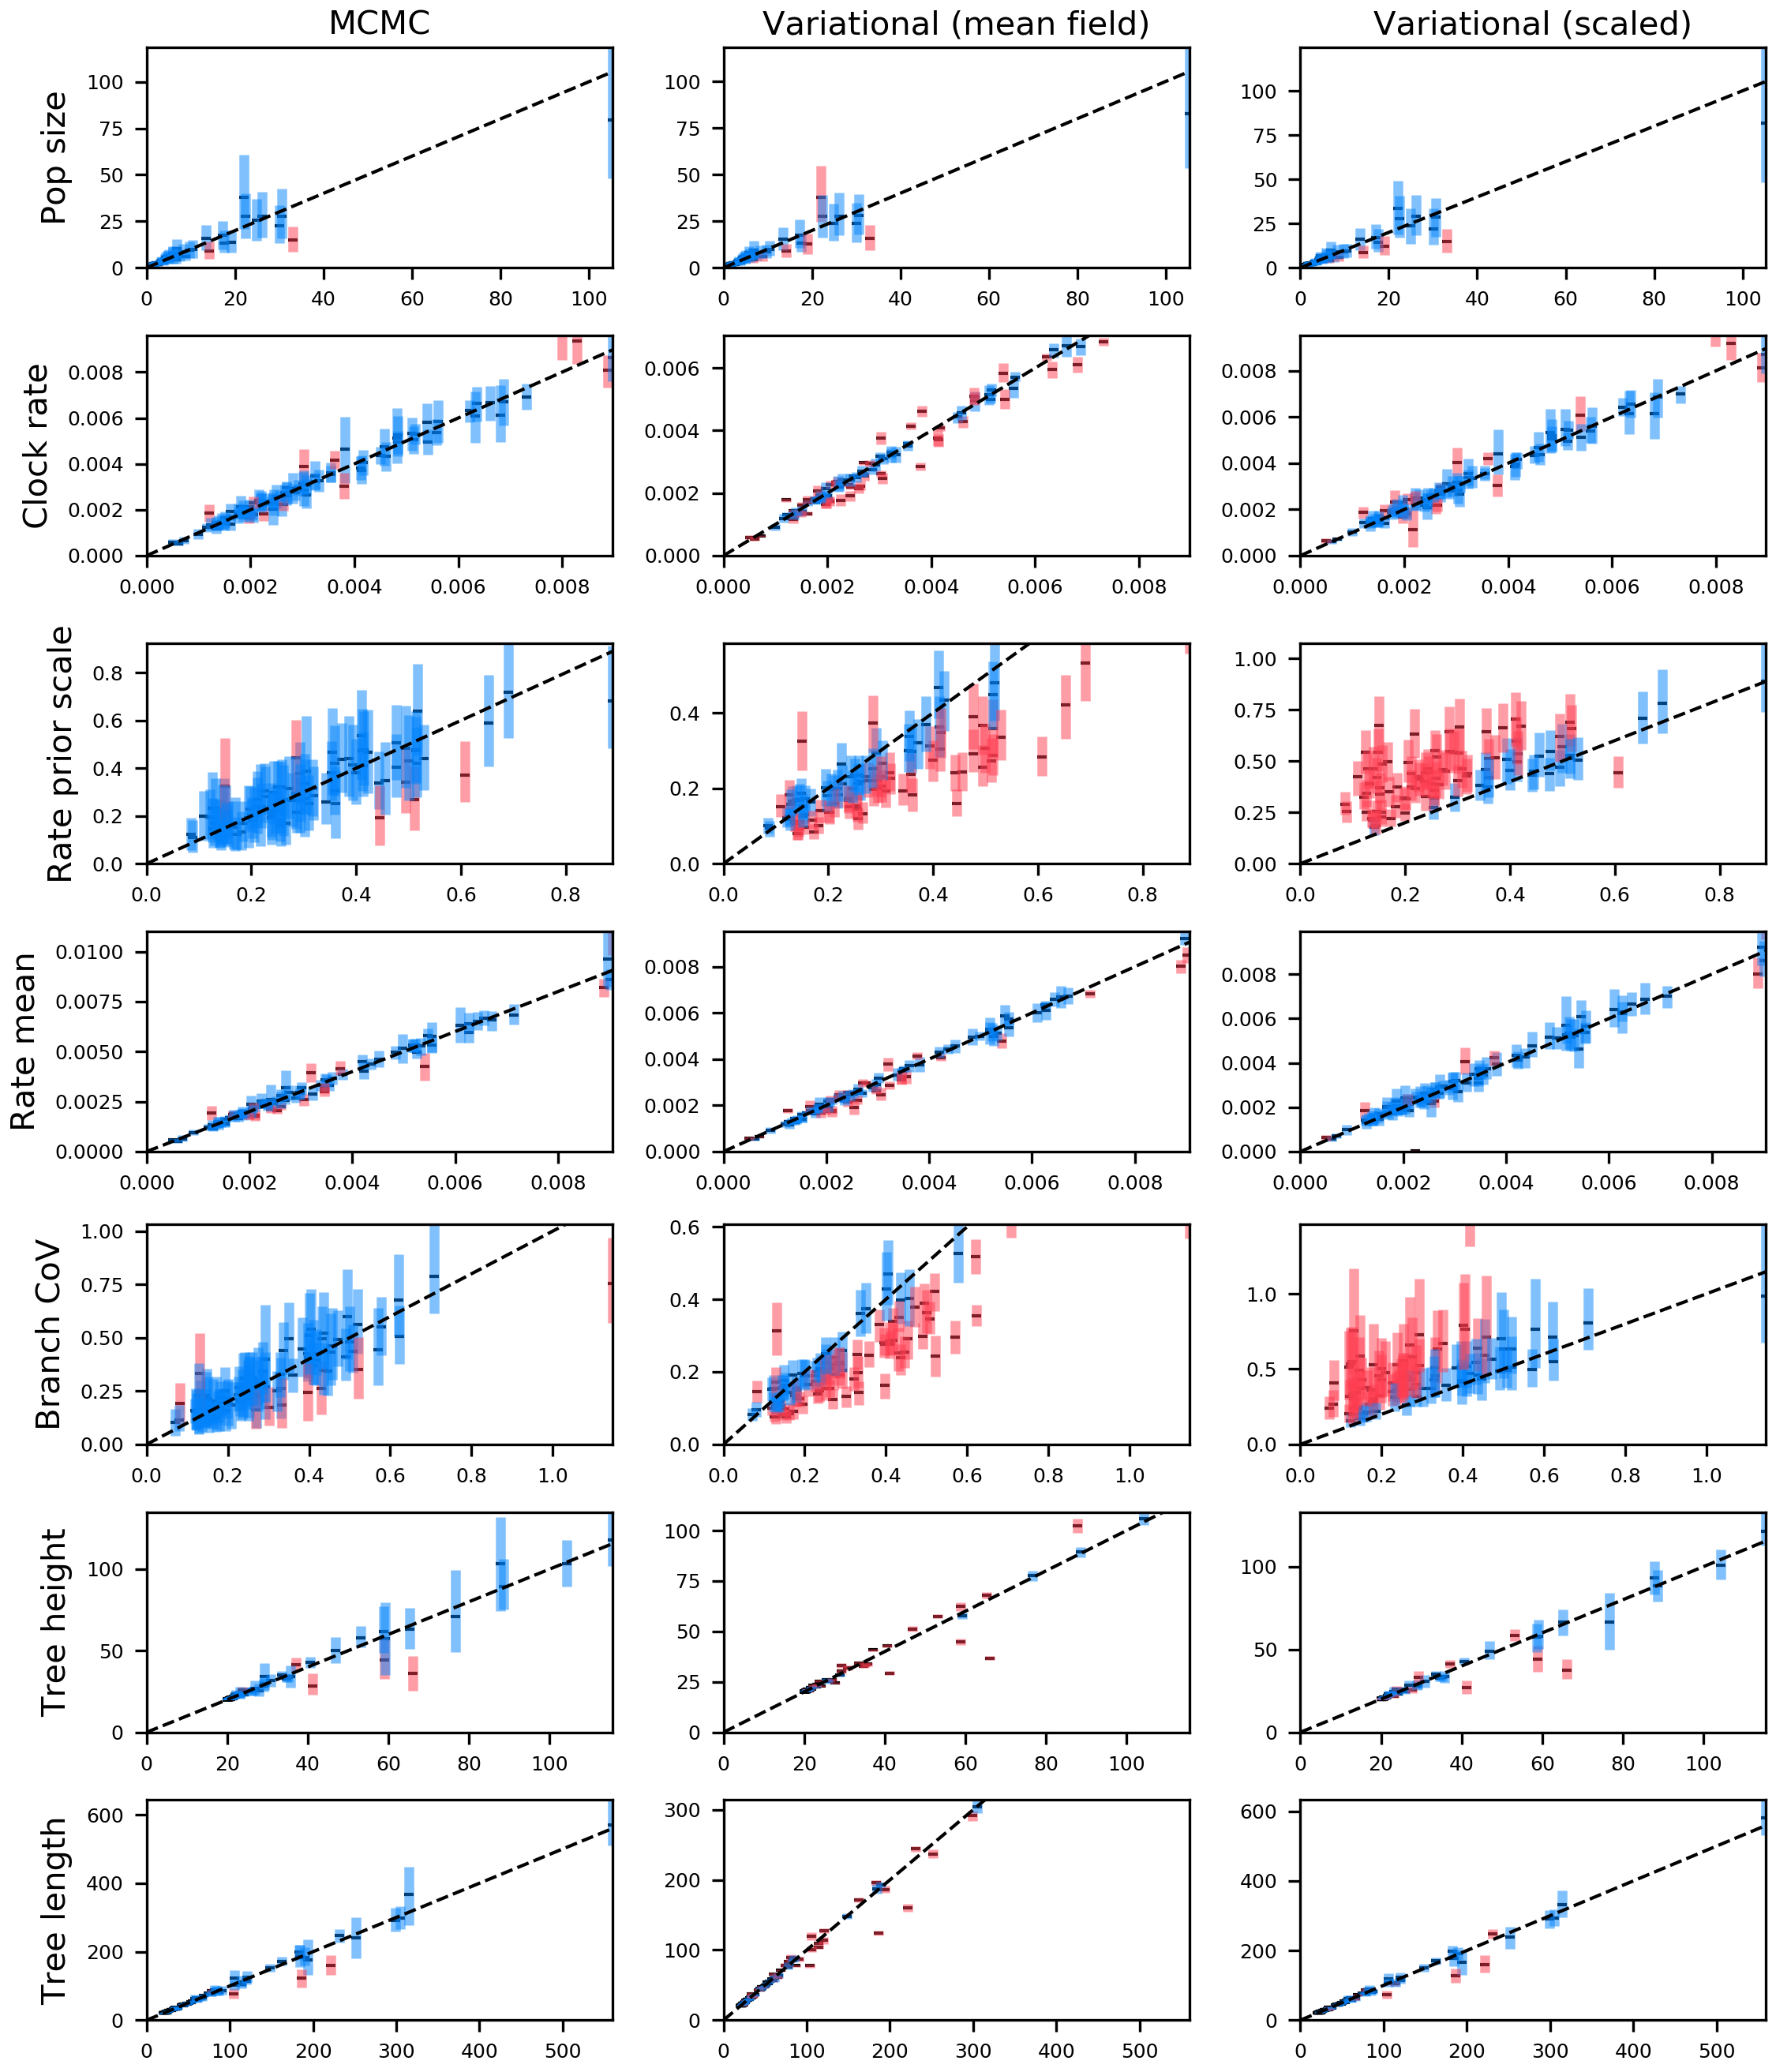
\includegraphics[width=\linewidth]{manuscript/figures/coverage}
    \caption{Results of simulation study}
    \label{fig:coverage}
\end{figure}
% Posterior comparison - mean field VS product VS MCMC fixed
% Performance evaluation - Variational vs MCMC - RSV dataset

\section*{Discussion}

\section*{Conclusions}

\section*{Supporting information}

% Include only the SI item label in the paragraph heading. Use the \nameref{label} command to cite SI items in the text.
\paragraph*{S1 Fig.}
\label{S1_Fig}
{\bf Bold the title sentence.} Add descriptive text after the title of the item (optional).

\section*{Acknowledgments}
Acknowledgments


\bibliography{main}

\end{document}
